\chapter{結論}
\label{conclusion}

本章では,本研究のまとめと今後の課題を示す.

\section{本研究のまとめ}
本研究では,IPv6シングルスタックネットワークにおけるIPv4サービス提供手法として,ステートレスアドレス変換を利用した"SIIT-DC"と呼ばれるネットワークデザインに注目し,冗長性や変更追従性の問題を解決するために,考えられるアプローチを比較した上で,動的経路制御プロトコルであるBGPを利用したアドレス変換テーブルの広告・更新プロトコルを設計した.

本手法を評価するために,OSS及び自作のを利用したPoCを実装し,30台のBR,2台のルートリフレクタ,最大600台のサーバからなる評価用ネットワークにて2つのシナリオからなる評価実験を行った.
本評価実験の結果,本手法がSIIT-DCの冗長性と変更追従性を改善するフィジビリティを十分に有することが明らかになった.

\section{よりスケーラブルなBGPコネクショントポロジについての検討}
本評価実験を通して,ルートリフレクタが保有するべきBGPコネクションの数が大きくなることが,IPv4サービス提供サーバの収容可能台数と変更追従性に影響を及ぼすことがわかっている.

これはBGPコネクショントポロジを階層的なものにすることで,よりスケーラブルに本提案手法を運用することが可能である.


第\ref{evaluation:environment}節で述べたように,本概念実証用ネットワークでは全てのIPv4サービス提供サーバ・BRを同一のルートリフレクタに接続する1層のフラットなBGPコネクショントポロジを採用していた.図\ref{fig:1layer_bgp_topology}に本評価環境におけるBGPコネクショントポロジを簡略化して示す.


\begin{figure}[h]
    \begin{center}
    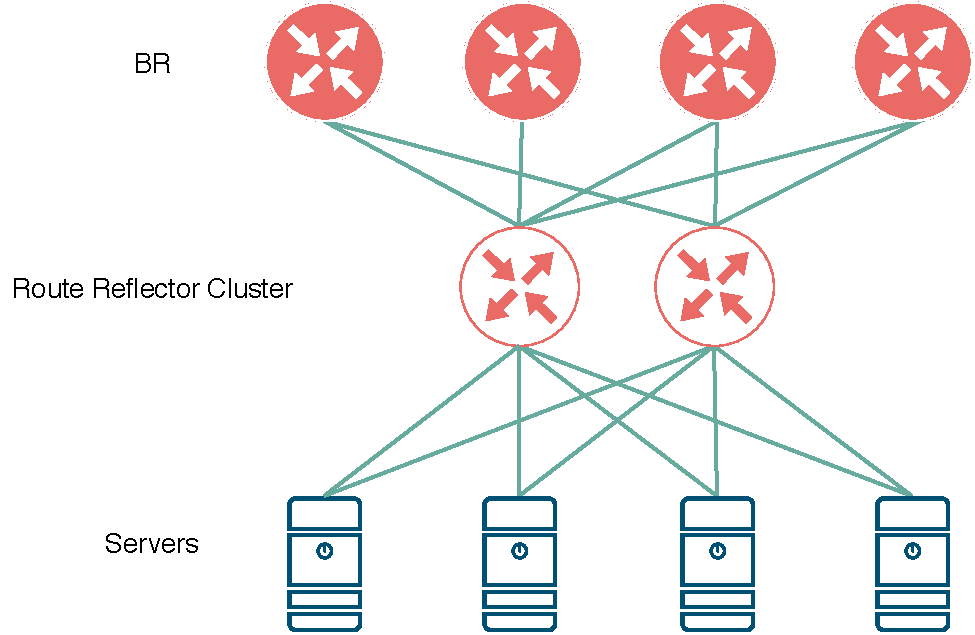
\includegraphics[width=12cm,pagebox=cropbox,clip]{img/1layer_bgp_topology.pdf}
    \end{center}
    \caption{1層のBGPコネクショントポロジ}
    \label{fig:1layer_bgp_topology}
\end{figure}

本評価環境と同じBGPコネクショントポロジを採用したIDCに於いて,ネットワーク全体で収容可能なIPv4サービス提供サーバ数$S_1$は式\ref{eq:1layer_max_connection}のように示すことが出来る.この時,BRの数を$B$,1台のルートリフレクタが収容可能なBGPピアの最大の数を$L_r$とする.

\begin{equation}
    S_1 = L_r - B
    \label{eq:1layer_max_connection}
\end{equation}


スケーラブルなBGPコネクショントポロジn例として,2層のルートリフレクタを採用したトポロジを図\ref{fig:2layer_bgp_topology}に示す.


\begin{figure}[h]
    \begin{center}
    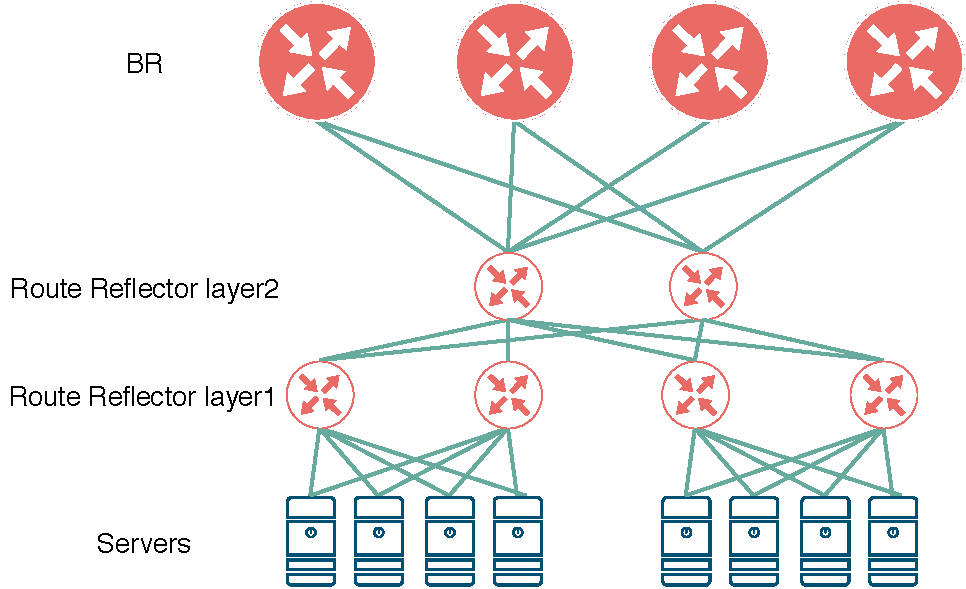
\includegraphics[width=12cm,pagebox=cropbox,clip]{img/2layer_bgp_topology.pdf}
    \end{center}
    \caption{2層のBGPコネクショントポロジ}
    \label{fig:2layer_bgp_topology}
\end{figure}


また,本トポロジーを採用したIDCネットワークにおける収容可能なサーバ数$S_2$は式\ref{eq:2layer_max_connection}示す.先に述べた1層のコネクショントポロジと同様にBRの数を$B$,1台のルートリフレクタが収容可能なBGPピアの最大の数を$L_r$とする.


\begin{equation}
    S_2 = L_r(L_r - B)
    \label{eq:2layer_max_connection}
\end{equation}


第\ref{evaluation:eval1:result}項で示したように,本提案手法においてネットワーク全体で収容可能なIPv4サービス提供サーバ数は600台程度であることが明らかになっている.
すなわち本評価環境においては$L_r=630$であることがわかるため,2層のBGPコネクショントポロジを採用したBR30台を有するネットワークでは,ルートリフレクタを水平的に展開することにより最大378000のIPv4サービス提供サーバを収容可能であると導出出来る.



このようにBGPコネクショントポロジを多層化することで,本提案手法のスケーラビリティをより高める事が可能になることがわかる.

同時に,本提案手法は数万台規模のサーバを抱える実際の商用ネットワークにおいても本提案手法を展開可能であると評価することが出来る.



% \subsection{EAMの集約}
% 本提案手法では,IPv4サービス提供サーバ自身がIPv4サービスアドレスを広告することを前提とした設計を行った.
% IPv4サービスアドレスを有するサーバ以外がEAMを複数集約して代理に広告するというユースケースを想定すると,BGPが利用するアドレスファミリの拡張仕様の設計が必要になると言える.


%%% Local Variables:
%%% mode: japanese-latex
%%% TeX-master: "../thesis"
%%% End:
